\documentclass[12pt,a4paper]{article}
\usepackage[utf8]{inputenc}
\usepackage[spanish]{babel}
\usepackage{amsmath}
\usepackage{amsfonts}
\usepackage{amssymb}	
\usepackage{makeidx}
\usepackage{graphicx}
\usepackage{lmodern}
\usepackage[usenames]{color}
\usepackage{multirow}
\usepackage[table,xcdraw]{xcolor}
\usepackage{lscape}
\usepackage{longtable}
\usepackage{graphicx}
%\usepackage{hyperref}
\usepackage{url}
%\usepackage{xcolor}
%\usepackage{titlesec}
%\usepackage{kpfonts}
\usepackage{colortbl}

%%%%
%para no cortar palabras por silabas
\usepackage[none]{hyphenat}

%internlineado

\usepackage{setspace}


\usepackage{blindtext}
\usepackage{hyperref}

\setlength{\parindent}{0pt}

\usepackage{color,hyperref}
\definecolor{darkblue}{rgb}{0.0667, 0.1255, 0.1922}
\hypersetup{colorlinks,breaklinks,
	linkcolor=darkblue,urlcolor=darkblue,
	anchorcolor=darkblue,citecolor=darkblue}
%%%%

\usepackage[table]{xcolor}
\usepackage[left=3cm,right=3cm,top=3cm,bottom=3cm]{geometry}

%%%%%%%%%%%%%%%%%%%%%%%%%

\usepackage{times}

\usepackage{color}
\definecolor{gray97}{gray}{.97}
\definecolor{gray75}{gray}{.75}
\definecolor{gray45}{gray}{.45}

\usepackage{listings}
\lstset{ frame=Ltb,
	framerule=0pt,
	aboveskip=0.5cm,
	framextopmargin=1pt,
	framexbottommargin=4pt,
	framexleftmargin=0.4cm,
	framesep=0pt,
	rulesep=.4pt,
	backgroundcolor=\color{gray97},
	rulesepcolor=\color{black},
	%
%
stringstyle=\ttfamily,
showstringspaces = false,
basicstyle=\small\ttfamily,
commentstyle=\color{gray45},
keywordstyle=\bfseries,
%
numbers=left,
numbersep=15pt,
numberstyle=\tiny,
numberfirstline = false,
breaklines=true,
}

% minimizar fragmentado de listados
\lstnewenvironment{listing}[1][]
{\lstset{#1}\pagebreak[0]}{\pagebreak[0]}

\lstdefinestyle{consola}
{basicstyle=\scriptsize\bf\ttfamily,
backgroundcolor=\color{gray75},
}

\lstdefinestyle{C}
{language=C,
}

%%%%%%%%%%%%%%%%%%%%%%%%%


%\titleformat{\chapter}[frame]
%{\LARGE\color{AzulClaro}}{\filright\chaptertitlename\ \thechapter}{20pt}{\Huge}

%\titleformat*{\section}{\Large\bfseries\color{blue}}

\title{\huge{Subjective Well-Being Data Task}}

\author{ 
	Jason Cruz\\ 
	\href{mailto:164468@unsaac.edu.pe}{164468@unsaac.edu.pe}
} 

\date{\ Setiembre, 2021}

\begin{document}
	\maketitle 
	
%\tableofcontents{}
	
\section*{{\textcolor[rgb]{0.0667, 0.1255, 0.1922}{Question 1}}}
	\subsection*{\normalsize{a) Load ratings.csv}}
	
	\noindent
	This is achieved using the following code:
	
	\begin{lstlisting}[language=Stata]
	import delimited using "${data}/ratings.csv", clear
	\end{lstlisting} 
	
	The working directory was previously defined. The complete steps are appreciated the Master Script.
	
	\subsection*{\normalsize{b) Report the number of unique respondents and the number of unique aspects in the data set}}
	
	\begin{table}[htbp]
		\resizebox{5 cm}{!}{%
			\begin{tabular}{lll}
				\hline
				\textbf{Variable} & \textbf{Obs} & \textbf{Unique} \\ \hline
				aspect            & 18189        & 17              \\ \hline
				worker            & 18189        & 1056            \\ \hline
			\end{tabular}%
		}
	\end{table} \\
	
	\subsection*{\normalsize{c) Check to see if each respondent has only rated each aspect once. If this is not true, only include the most recent observation and report the number of observations you have dropped.}}
	
	\noindent
	The following command generates a unique id group, at the same time, it orders by "time variable"; by default the time is ordered from most recent to least recent. It also generates an empty value that corresponds to the oldest time and duplicate aspect. All the requirements of the question were met.
	
	\begin{lstlisting}[language=Stata]
	bysort worker aspect (time) : gen newid = 1 if _n==1
	\end{lstlisting} 
	
	\noindent
	The commands below count how many values ​​are not
	they corresponded to a unique aspect and drop these values.
	
	\begin{lstlisting}[language=Stata]
	count if newid == .	
	drop if newid == .
	\end{lstlisting}
	
	\noindent
	The command returns the number of observations I have dropped.
	
	\begin{lstlisting}[language=Stata]
		(237 observations deleted)
	\end{lstlisting}
	
	\subsection*{\normalsize{d) Calculate the average rating for each respondent. We will call this measure subjective riches. Report the minimum, 25th percentile, 50th percentile, 75th percentile, and maximum subjective riches value.}}	
	
	\begin{itemize}
		\item The average score of each respondent is calculated using the code. 
	\noindent	
	\begin{lstlisting}[language=Stata]
	egen subjective_riches = mean(rating),///
	by(worker)
	\end{lstlisting}
		
		\item The minimum, 25th percentile, 50th percentile, 75th percentile, and maximum subjective riches value.
	
			\begin{table}[htbp]
				\resizebox{11 cm}{!}{%
					\begin{tabular}{llllll}
						\hline
						\textbf{Variable} & \textbf{min} & \textbf{p25} & \textbf{p50} & \textbf{p75} & \textbf{max} \\ \hline
						Subjective Riches & 5.764706     & 49.05882     & 61.44118     & 75.08823     & 100          \\ \hline
					\end{tabular}%
				}
			\end{table}
	
	\end{itemize}
	
\section*{{\textcolor[rgb]{0.0667, 0.1255, 0.1922}{Question 2}}}
	\subsection*{\normalsize{a) Load demographics.csv}}
	
	\noindent
	This is achieved using the following code:
	
	\begin{lstlisting}[language=Stata]
	import delimited using "${data}/demographics.csv", clear
	\end{lstlisting}
	
	\subsection*{\normalsize{b) Report the number of rows and check to see if it is the same as the number of unique respondents you calculated in question 1.}}
	
	\noindent
	I use the two commands below to generate the number of rows and then report, respectively.
	
	\begin{lstlisting}[language=Stata]
	scalar number_rows = c(N)
	scalar list  number_rows
	\end{lstlisting}
	
	Evidently, this is the same as the number of unique respondents I calculated in question 1.
	
	\subsection*{\normalsize{c) Merge the subjective riches data from question 1 with the demographics data.}}
	
	\noindent
	This is possible with the command
	\begin{lstlisting}[language=Stata]
	merge 1:m worker using  "${data}/ratings.dta", ///
	nogen keepusing(time rating subjective_riches aspect)
	\end{lstlisting}

\begin{table}[htbp]
	\resizebox{4 cm}{!}{%
		\begin{tabular}{ll}
			\hline
			\textbf{Result} & \textbf{\# of obs.} \\ \hline
			not matched     & 0                   \\ \hline
			matched         & 17,952              \\ \hline
		\end{tabular}%
	}
\end{table}

	\subsection*{\normalsize{d) Regress (with OLS) subjective riches on income and report the results.}}
	
	\begin{center}
		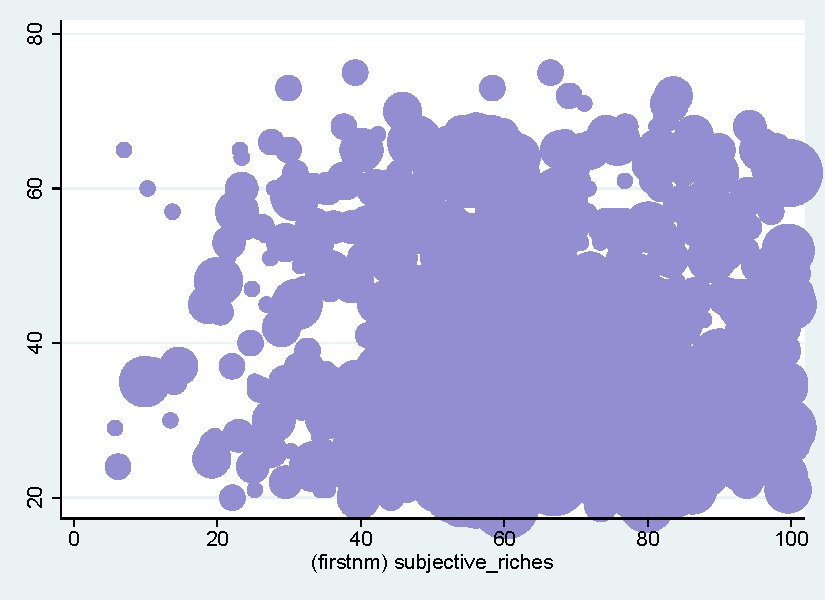
\includegraphics[width=1\linewidth]{"C:/Users/PC/Documents/BID-Columbia/Data Task/figures/model_1.pdf"}
	\end{center}
	
	{
\def\sym#1{\ifmmode^{#1}\else\(^{#1}\)\fi}
\begin{tabular}{l*{1}{cc}}
\hline\hline
            &\multicolumn{1}{c}{(1)}         &            \\
            &  Coef./S.E.         &     p-value\\
\hline
income      &        0.00\sym{***}&        0.00\\
            &        0.00         &            \\
Const       &       56.28\sym{***}&        0.00\\
            &        0.25         &            \\
\hline
R-cuadrado  &        0.04         &            \\
N. de obs.  &    17952.00         &            \\
\hline\hline
\multicolumn{3}{l}{\footnotesize \sym{*} \(p<0.05\), \sym{**} \(p<0.01\), \sym{***} \(p<0.001\)}\\
\end{tabular}
}

	
	\begin{itemize}
		\item Interpret the results. What is the relationship between income and subjective riches? (Max
		100 words).
		
		There is a very weak positive relationship. The coefficient 0.0000927 (significant by p-value) is interpreted as: for each additional monetary unit that the respondent receives, his or her score in aspects of well-being increases by 0.0000927 points. This low value means that there are other determinants other than income that better explain the differences in aspects of well-being (such as health, happiness, etc.). In addition, being a bivariate model without controls, the correlation is weak with a very low R squared, although this is not a dazzling indicator in this analysis, we are practically facing an ad hoc model.
		
	\end{itemize}
	\subsection*{\normalsize{e) Regress (with OLS) subjective riches on income with controls for age, $age^{2}$ (age squared), gender, level of education, and race.}}
	
	{
\def\sym#1{\ifmmode^{#1}\else\(^{#1}\)\fi}
\begin{tabular}{l*{2}{cc}}
\hline\hline
            &\multicolumn{1}{c}{(1)}         &            &\multicolumn{1}{c}{(2)}         &            \\
            &  Coef./S.E.         &     p-value&  Coef./S.E.         &     p-value\\
\hline
income      &        0.00\sym{***}&        0.00&        0.00\sym{***}&        0.00\\
            &        0.00         &            &        0.00         &            \\
Const       &       56.28\sym{***}&        0.00&       68.66\sym{***}&        0.00\\
            &        0.25         &            &        1.89         &            \\
age         &                     &            &       -0.35\sym{***}&        0.00\\
            &                     &            &        0.07         &            \\
age\_squared &                     &            &        0.00\sym{***}&        0.00\\
            &                     &            &        0.00         &            \\
0.male      &                     &            &        0.00         &           .\\
            &                     &            &           .         &            \\
1.male      &                     &            &        2.57\sym{***}&        0.00\\
            &                     &            &        0.29         &            \\
1.education\_new&                     &            &        0.00         &           .\\
            &                     &            &           .         &            \\
2.education\_new&                     &            &       -6.90\sym{***}&        0.00\\
            &                     &            &        1.33         &            \\
3.education\_new&                     &            &       -7.61\sym{***}&        0.00\\
            &                     &            &        1.27         &            \\
4.education\_new&                     &            &       -5.68\sym{***}&        0.00\\
            &                     &            &        1.49         &            \\
5.education\_new&                     &            &       -4.55\sym{***}&        0.00\\
            &                     &            &        1.27         &            \\
6.education\_new&                     &            &       -7.28\sym{***}&        0.00\\
            &                     &            &        1.35         &            \\
7.education\_new&                     &            &       -2.39         &        0.12\\
            &                     &            &        1.54         &            \\
1.race\_new  &                     &            &        0.00         &           .\\
            &                     &            &           .         &            \\
2.race\_new  &                     &            &        7.11\sym{***}&        0.00\\
            &                     &            &        0.70         &            \\
3.race\_new  &                     &            &       -2.33\sym{***}&        0.00\\
            &                     &            &        0.55         &            \\
4.race\_new  &                     &            &       -2.02\sym{***}&        0.00\\
            &                     &            &        0.56         &            \\
5.race\_new  &                     &            &       -0.67         &        0.21\\
            &                     &            &        0.54         &            \\
6.race\_new  &                     &            &        8.41\sym{***}&        0.00\\
            &                     &            &        1.62         &            \\
\hline
R-cuadrado  &        0.04         &            &        0.06         &            \\
N. de obs.  &    17952.00         &            &    17935.00         &            \\
\hline\hline
\multicolumn{5}{l}{\footnotesize \sym{*} \(p<0.05\), \sym{**} \(p<0.01\), \sym{***} \(p<0.001\)}\\
\end{tabular}
}

	
	\begin{itemize}
		\item Interpret the results. (Max 150 words).
	\end{itemize}

The model has improved since the specification, it is more interesting the relationships of the control variables with subjective riches according to the results. For example, the negative coefficient of age (significant) shows that each additional year represents -0.35 points on the aspects of well-being, while the coefficient of age\_squared shows that at a certain age (many years of life) the respondents value more the aspects of well-being, older adults probably rate well-being aspects higher than young people. Likewise, being a male respondent means scoring the aspects of well-being with 2.57 points more than women. On the other hand, for the most part, the categories of the variables education and race score the aspects of well-being less.

	\subsection*{\normalsize{f) Imagine you were also given each respondent’s household size.(Max 100 words).}}
	
	{
\def\sym#1{\ifmmode^{#1}\else\(^{#1}\)\fi}
\begin{tabular}{l*{3}{cc}}
\hline\hline
            &\multicolumn{1}{c}{(1)}         &            &\multicolumn{1}{c}{(2)}         &            &\multicolumn{1}{c}{(3)}         &            \\
            &  Coef./S.E.         &     p-value&  Coef./S.E.         &     p-value&  Coef./S.E.         &     p-value\\
\hline
income      &        0.00\sym{***}&        0.00&        0.00\sym{***}&        0.00&                     &            \\
            &        0.00         &            &        0.00         &            &                     &            \\
Const       &       56.28\sym{***}&        0.00&       68.66\sym{***}&        0.00&     7843.48\sym{*}  &        0.04\\
            &        0.25         &            &        1.89         &            &     3830.02         &            \\
age         &                     &            &       -0.35\sym{***}&        0.00&      243.69         &        0.10\\
            &                     &            &        0.07         &            &      149.33         &            \\
age\_squared &                     &            &        0.00\sym{***}&        0.00&       -4.46\sym{**} &        0.01\\
            &                     &            &        0.00         &            &        1.67         &            \\
0.male      &                     &            &        0.00         &           .&        0.00         &           .\\
            &                     &            &           .         &            &           .         &            \\
1.male      &                     &            &        2.57\sym{***}&        0.00&      616.53         &        0.29\\
            &                     &            &        0.29         &            &      583.87         &            \\
1.education\_new&                     &            &        0.00         &           .&        0.00         &           .\\
            &                     &            &           .         &            &           .         &            \\
2.education\_new&                     &            &       -6.90\sym{***}&        0.00&     9084.86\sym{***}&        0.00\\
            &                     &            &        1.33         &            &     2203.85         &            \\
3.education\_new&                     &            &       -7.61\sym{***}&        0.00&    17652.57\sym{***}&        0.00\\
            &                     &            &        1.27         &            &     2141.13         &            \\
4.education\_new&                     &            &       -5.68\sym{***}&        0.00&    49033.29\sym{***}&        0.00\\
            &                     &            &        1.49         &            &     2580.31         &            \\
5.education\_new&                     &            &       -4.55\sym{***}&        0.00&    29767.44\sym{***}&        0.00\\
            &                     &            &        1.27         &            &     2141.46         &            \\
6.education\_new&                     &            &       -7.28\sym{***}&        0.00&    49755.59\sym{***}&        0.00\\
            &                     &            &        1.35         &            &     2410.27         &            \\
7.education\_new&                     &            &       -2.39         &        0.12&    54239.02\sym{***}&        0.00\\
            &                     &            &        1.54         &            &     3910.63         &            \\
1.race\_new  &                     &            &        0.00         &           .&        0.00         &           .\\
            &                     &            &           .         &            &           .         &            \\
2.race\_new  &                     &            &        7.11\sym{***}&        0.00&    -2116.96         &        0.18\\
            &                     &            &        0.70         &            &     1586.42         &            \\
3.race\_new  &                     &            &       -2.33\sym{***}&        0.00&    -2897.10\sym{*}  &        0.01\\
            &                     &            &        0.55         &            &     1130.09         &            \\
4.race\_new  &                     &            &       -2.02\sym{***}&        0.00&    -5405.79\sym{***}&        0.00\\
            &                     &            &        0.56         &            &      812.69         &            \\
5.race\_new  &                     &            &       -0.67         &        0.21&    12723.95\sym{***}&        0.00\\
            &                     &            &        0.54         &            &     1428.59         &            \\
6.race\_new  &                     &            &        8.41\sym{***}&        0.00&   -24345.41\sym{***}&        0.00\\
            &                     &            &        1.62         &            &     2995.12         &            \\
subjective\_riches&                     &            &                     &            &      350.85\sym{***}&        0.00\\
            &                     &            &                     &            &       13.95         &            \\
household\_size&                     &            &                     &            &      165.15         &        0.40\\
            &                     &            &                     &            &      197.27         &            \\
\hline
R-cuadrado  &        0.04         &            &        0.06         &            &        0.14         &            \\
N. de obs.  &    17952.00         &            &    17935.00         &            &    17935.00         &            \\
\hline\hline
\multicolumn{7}{l}{\footnotesize \sym{*} \(p<0.05\), \sym{**} \(p<0.01\), \sym{***} \(p<0.001\)}\\
\end{tabular}
}

	
	 \textbf{How would you change your analysis above in light of this new information?}\\[0.5 cm]	
	 Coefficients of the continuous and categorical controls have changed abruptly, even changed sign. It is that to say, the "household size" would significantly influence on model. If we had "household size" in data, the results would change as this simulation shows.
	 As the questions (so far) asked us for specific tasks, I were unable to carry out a more rigorous analysis. To improve analysis, I should set a better specification and  work more on the proxy. Then the estimation would be simpler. On the other hand, the R squared is not reliable. Basically, we cannot see causality but only correlation.
	 
\section*{{\textcolor[rgb]{0.0667, 0.1255, 0.1922}{Question 3}}}

Your PI is giving a presentation to a health-policy audience, and she would like to display a figure that illustrates the relationship between subjective ratings of health, income, and age. She has asked you to produce a single scatterplot that conveys the relationship between all three variables.

	\subsection*{\normalsize{a) List the steps you would take to produce the scatterplot. Remember}}
	\begin{itemize}
		\item Any individual/average rating data in your plot should be for aspects related to health.
		\item All three variables should be featured in some way on the plot.
		\item The figure should readable, effectively convey the information through visuals, and preferably
		be intuitively understandable to an audience that has limited familiarity with the
		survey and your data set.
	\end{itemize}

\textbf{Steps}

\begin{enumerate}
	\item I generate a new variable that contains only health aspects
	\item Sort by age
	\item Seperate age variable, by health_aspect
	\item Use twoway command to include several options in the graph, this means, of course, include three variables where one of them represents the size of the bubbles.
	\item Save as "scatter_plot" and export graphic as PDF.
\end{enumerate}

	\subsection*{\normalsize{b) Produce and save the scatterplot (or if you prefer, up to two proposals for alternative scatterplots).}}
	
	The graph was produced by twoway command and saved as "scatter plot" as pdf.
	
	I used the following command within the graph's own options.
	
	\begin{lstlisting}[language=Stata]
	name(scatter_plot, replace)
	\end{lstlisting}

	I used below command to export as pdf.
	
	\begin{lstlisting}[language=Stata]
	graph export "${figures}\model_1.pdf", as(pdf) replace
	\end{lstlisting}
	
	\textit{Note: I don't show my graph because I didn't get the result I expected}
	
	\subsection*{\normalsize{c) From a policy perspective, understanding the determinants of well-being is an important question. Describe the ways in which your regressions in the previous question and your scatterplot(s) help or do not help answer this question. Think about your proxy for well-being (subjective ratings) as well as the specification of your regressions. (Max 250 words)}}
	
	In my opinion, the analysis previously developed is not enough to answer such an important question as “determinants of well-being”.
	Firstly, I performed a bivariate regression between subjective riches and income. This regression is not rigorous since causality is not possible; however, for this to make sense, I chose the subjective riches as a response variable and income as explanatory; doing it the other way around had no background since my variable of interest is subjective riches. It was interesting to ask the question: Will the welfare of respondents increase with higher income? But this question cannot be answered with such a simple specification.
	Secondly, when regress with continuous and categorical control variables, they latter looked more interesting since their coefficients showed higher magnitude marginal effects on the main variable. However, from my point of view, I should have modeled differently than OLS because the response variable in this case, although continuous, is limited; it is that to say, the OLS estimate does not fit the data very well. My alternative would be to model with logit or use other multinomial models.
	Finally, it may be useful to think of a welfare proxy as a more specific dependent variable (using another estimation method), as requested in question 3 f) (only for health aspects) because it is better to isolate effects for modeling.\\[0.8 cm]

	
	\textit{Visit \href{"https://github.com/JasonCruz18/Subjective_Well-Being_Data_Task-BID-Columbia/network" }{Network graph (GitHub)} to know the sequence of my work to answer the questions of this great task}
	
\end{document}	